%%%%% Set up %%%%%

% Set document style and font size
\documentclass[12pt]{article}\usepackage[]{graphicx}\usepackage[]{color}
%% maxwidth is the original width if it is less than linewidth
%% otherwise use linewidth (to make sure the graphics do not exceed the margin)
\makeatletter
\def\maxwidth{ %
  \ifdim\Gin@nat@width>\linewidth
    \linewidth
  \else
    \Gin@nat@width
  \fi
}
\makeatother

\definecolor{fgcolor}{rgb}{0.345, 0.345, 0.345}
\newcommand{\hlnum}[1]{\textcolor[rgb]{0.686,0.059,0.569}{#1}}%
\newcommand{\hlstr}[1]{\textcolor[rgb]{0.192,0.494,0.8}{#1}}%
\newcommand{\hlcom}[1]{\textcolor[rgb]{0.678,0.584,0.686}{\textit{#1}}}%
\newcommand{\hlopt}[1]{\textcolor[rgb]{0,0,0}{#1}}%
\newcommand{\hlstd}[1]{\textcolor[rgb]{0.345,0.345,0.345}{#1}}%
\newcommand{\hlkwa}[1]{\textcolor[rgb]{0.161,0.373,0.58}{\textbf{#1}}}%
\newcommand{\hlkwb}[1]{\textcolor[rgb]{0.69,0.353,0.396}{#1}}%
\newcommand{\hlkwc}[1]{\textcolor[rgb]{0.333,0.667,0.333}{#1}}%
\newcommand{\hlkwd}[1]{\textcolor[rgb]{0.737,0.353,0.396}{\textbf{#1}}}%
\let\hlipl\hlkwb

\usepackage{framed}
\makeatletter
\newenvironment{kframe}{%
 \def\at@end@of@kframe{}%
 \ifinner\ifhmode%
  \def\at@end@of@kframe{\end{minipage}}%
  \begin{minipage}{\columnwidth}%
 \fi\fi%
 \def\FrameCommand##1{\hskip\@totalleftmargin \hskip-\fboxsep
 \colorbox{shadecolor}{##1}\hskip-\fboxsep
     % There is no \\@totalrightmargin, so:
     \hskip-\linewidth \hskip-\@totalleftmargin \hskip\columnwidth}%
 \MakeFramed {\advance\hsize-\width
   \@totalleftmargin\z@ \linewidth\hsize
   \@setminipage}}%
 {\par\unskip\endMakeFramed%
 \at@end@of@kframe}
\makeatother

\definecolor{shadecolor}{rgb}{.97, .97, .97}
\definecolor{messagecolor}{rgb}{0, 0, 0}
\definecolor{warningcolor}{rgb}{1, 0, 1}
\definecolor{errorcolor}{rgb}{1, 0, 0}
\newenvironment{knitrout}{}{} % an empty environment to be redefined in TeX

\usepackage{alltt}

% File path to resources (style file etc)
\newcommand{\locRepo}{csas-style}

% Style file for DFO Technical Reports
\usepackage{\locRepo/tech-report}

% header-includes from R markdown entry


%%%%% Variables %%%%%

% New definitions: Title, year, report number, authors
% Protect lower case words (i.e., species names) in \Addlcwords{}, in "TechReport.sty"
\newcommand{\trTitle}{Title Here (\emph{Latin Species Name})}
\newcommand{\trYear}{20XX}
\newcommand{\trReportNum}{nnn}
% Optional
\newcommand{\trAuthFootA}{Email: \href{mailto:First.Author@dfo-mpo.gc.ca}{\nolinkurl{First.Author@dfo-mpo.gc.ca}} \textbar{} telephone: (250) 756-5555}
\newcommand{\trAuthsLong}{First. M. Last\textsuperscript{1} and Alex B. Smith\textsuperscript{2}}
\newcommand{\trAuthsBack}{Last, F.M. and Smith, A.B.}

% New definition: Address
\newcommand{\trAddy}{\textsuperscript{1}Pacific Biological Station\\
Fisheries and Oceans Canada, 3190 Hammond Bay Road\\
Nanaimo, British Columbia, V9T 6N7, Canada\\
\textsuperscript{2}Far, far away\\
Another Galaxy}

% Abstract
\newcommand{\trAbstract}{Here is the abstract text. Lorem ipsum dolor sit amet, consectetur adipisicing elit, sed do eiusmod tempor incididunt ut labore et dolore magna aliqua. Ut enim ad minim veniam, quis nostrud exercitation ullamco laboris nisi ut aliquip ex ea commodo consequat. Duis aute irure dolor in reprehenderit in voluptate velit esse cillum dolore eu fugiat nulla pariatur. Excepteur sint occaecat cupidatat non proident, sunt in culpa qui officia deserunt mollit anim id est laborum.}

% Resume (i.e., French abstract)
\newcommand{\trResume}{Voici le résumé. Lorem ipsum dolor sit amet, consectetur adipisicing elit, sed do eiusmod tempor incididunt ut labore et dolore magna aliqua. Ut enim ad minim veniam, quis nostrud exercitation ullamco laboris nisi ut aliquip ex ea commodo consequat. Duis aute irure dolor in reprehenderit in voluptate velit esse cillum dolore eu fugiat nulla pariatur. Excepteur sint occaecat cupidatat non proident, sunt in culpa qui officia deserunt mollit anim id est laborum.}

%%%%% Start %%%%%

% Start the document
\IfFileExists{upquote.sty}{\usepackage{upquote}}{}
\begin{document}

%%%% Front matter %%%%%

% Add the first few pages
\frontmatter

%%%%% Drafts %%%%%

%\linenumbers  % Line numbers
%\onehalfspacing  % Extra space between lines
\renewcommand{\headrulewidth}{0.5pt}  % Header line
\renewcommand{\footrulewidth}{0.5pt}  % footer line
%\pagestyle{fancy}\fancyhead[c]{Draft: Do not cite or circulate}  % Header text

%%%%% Main document %%%%%
\hypertarget{introduction}{%
\section{Introduction}\label{introduction}}

A reference (Edwards et al. \protect\hyperlink{ref-edwards2013}{2014}).
\begin{equation}
  1 + 1
  \label{eq:test}
\end{equation}
See Appendix~\ref{app:first-appendix}. See Equation \eqref{eq:test}.

\hypertarget{methods}{%
\section{Methods}\label{methods}}
\begin{figure}[htb]

{\centering \pdftooltip{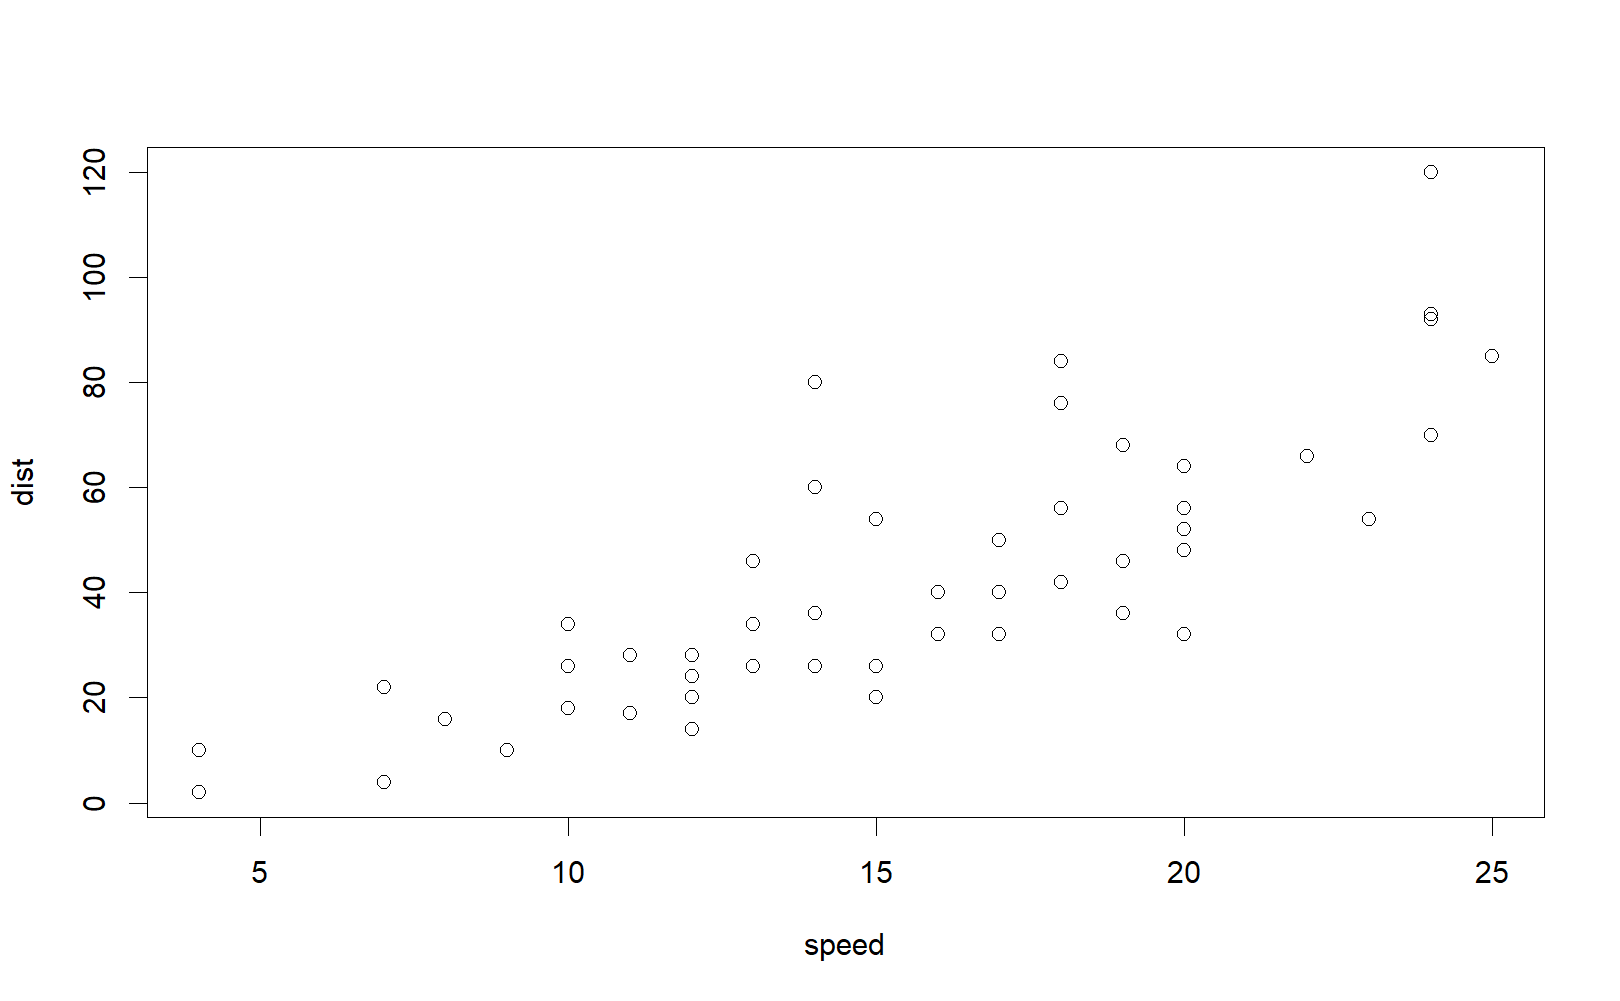
\includegraphics[width=6in]{knitr-figs-pdf/testfig-1}}{Figure \ref{fig:testfig}} 

}

\caption{Test figure with a caption will be numbered automatically.}\label{fig:testfig}
\end{figure}
\begin{longtable}[]{@{}crr@{}}
\caption{\label{tab:testtab}Test table with a caption will be numbered automatically.}\tabularnewline
\toprule
Year & Value 1 & Value 2\tabularnewline
\midrule
\endfirsthead
\toprule
Year & Value 1 & Value 2\tabularnewline
\midrule
\endhead
2018 & 1.12 & 31.9\tabularnewline
2019 & 2.32 & 2.8\tabularnewline
2020 & 3.67 & 112.2\tabularnewline
\bottomrule
\end{longtable}
See Table~\ref{tab:testtab} for the example table.

See Figure~\ref{fig:testfig} for the example figure.

\clearpage

\begingroup\fontsize{8}{10}\selectfont
\begin{landscape}
\begin{longtable}[t]{rrrrrrrrrrrrrrrr}
\caption{\label{tab:widelong}A long and wide table}\\
\toprule
\textbf{Year} & \textbf{1} & \textbf{2} & \textbf{3} & \textbf{4} & \textbf{5} & \textbf{6} & \textbf{7} & \textbf{8} & \textbf{9} & \textbf{10} & \textbf{11} & \textbf{12} & \textbf{13} & \textbf{14} & \textbf{15}\\
\midrule
\endfirsthead
\caption*{}\\
\toprule
\textbf{Year} & \textbf{1} & \textbf{2} & \textbf{3} & \textbf{4} & \textbf{5} & \textbf{6} & \textbf{7} & \textbf{8} & \textbf{9} & \textbf{10} & \textbf{11} & \textbf{12} & \textbf{13} & \textbf{14} & \textbf{15}\\
\midrule
\endhead
\
\endfoot
\bottomrule
\endlastfoot
1 & 21.6178 & 20.1295 & 18.2247 & 19.2058 & 18.6856 & 20.6018 & 20.7022 & 20.0093 & 22.2372 & 18.4420 & 19.4353 & 19.9990 & 18.9813 & 20.1281 & 19.8729\\
2 & 20.0534 & 21.1817 & 18.5944 & 20.2825 & 20.2597 & 19.6946 & 20.4135 & 19.8707 & 17.8460 & 20.2939 & 21.1135 & 19.9190 & 19.9430 & 21.6441 & 21.6085\\
3 & 19.4333 & 21.3081 & 19.9969 & 20.2032 & 22.5140 & 18.7517 & 19.4386 & 19.8504 & 19.1529 & 21.2822 & 19.7153 & 19.4668 & 20.3942 & 19.9922 & 21.3550\\
4 & 18.3408 & 18.5514 & 21.3580 & 19.5726 & 21.5300 & 20.0086 & 21.2857 & 19.2445 & 19.8217 & 20.6390 & 20.6495 & 21.7198 & 20.0502 & 19.1941 & 21.2961\\
5 & 18.1814 & 22.1055 & 19.5871 & 18.6146 & 19.5478 & 19.6533 & 20.6274 & 22.9447 & 22.3047 & 18.9667 & 20.1152 & 19.3458 & 19.3742 & 21.2943 & 21.0855\\
6 & 20.7234 & 20.7383 & 19.3042 & 20.2618 & 20.8808 & 20.9381 & 18.3407 & 21.2402 & 18.5909 & 19.8155 & 18.7426 & 18.3683 & 21.3541 & 20.5469 & 18.3046\\
7 & 19.3568 & 20.9995 & 17.3131 & 19.1832 & 21.1786 & 19.1968 & 20.9338 & 19.7675 & 21.0037 & 21.5813 & 21.0543 & 19.7722 & 19.6167 & 18.8485 & 18.4863\\
8 & 20.2014 & 21.2587 & 18.9522 & 20.5919 & 20.3179 & 21.4686 & 18.7227 & 19.6557 & 21.0472 & 20.8752 & 17.9806 & 19.9282 & 20.0511 & 19.5993 & 19.8529\\
9 & 21.4435 & 20.1873 & 20.1873 & 19.1906 & 19.9381 & 21.0880 & 20.1836 & 21.2459 & 19.4071 & 19.4897 & 18.8653 & 20.3168 & 18.6902 & 20.8721 & 20.2152\\
10 & 19.4194 & 19.1179 & 21.3360 & 19.5601 & 19.9840 & 18.6194 & 22.5557 & 18.9146 & 20.2431 & 19.9632 & 18.4539 & 20.7648 & 20.7802 & 19.2858 & 20.7189\\
11 & 18.1900 & 20.4187 & 19.8977 & 19.7836 & 21.0801 & 21.0707 & 22.0464 & 19.2979 & 19.7503 & 19.5144 & 18.5818 & 20.6899 & 19.2463 & 18.1553 & 19.1921\\
12 & 18.7288 & 19.4686 & 20.2336 & 20.7794 & 20.4016 & 19.7297 & 20.1056 & 19.0834 & 20.9215 & 20.1006 & 20.5834 & 19.5771 & 20.7778 & 20.5272 & 19.8871\\
13 & 21.8019 & 19.0502 & 19.4613 & 20.3043 & 20.8592 & 21.8891 & 20.6820 & 18.1819 & 21.4437 & 21.1477 & 18.2239 & 18.7397 & 19.1430 & 20.6131 & 20.1633\\
14 & 19.1860 & 20.1448 & 19.7488 & 20.5390 & 19.8176 & 17.8456 & 21.2060 & 19.0380 & 19.5083 & 20.5180 & 21.3301 & 20.1858 & 19.8261 & 19.6549 & 20.3129\\
15 & 18.9644 & 20.7491 & 19.7976 & 20.1104 & 19.2499 & 19.3192 & 20.1681 & 20.9207 & 18.6619 & 20.0958 & 21.2389 & 20.1626 & 19.9025 & 20.8171 & 19.5787\\
16 & 20.1942 & 18.6022 & 22.2448 & 19.2975 & 19.5669 & 19.7359 & 19.0267 & 19.7111 & 19.6187 & 20.4265 & 20.3918 & 19.8101 & 20.0657 & 21.6645 & 18.4275\\
17 & 19.7300 & 19.3048 & 19.4279 & 18.7961 & 21.6179 & 20.4852 & 20.8313 & 20.7122 & 20.5052 & 21.1359 & 17.8779 & 21.5905 & 19.2744 & 20.6282 & 19.7444\\
18 & 20.4725 & 21.7943 & 19.0768 & 20.1229 & 19.1550 & 20.6869 & 19.5054 & 21.1135 & 19.1624 & 19.7829 & 19.7878 & 21.0020 & 18.7468 & 20.7448 & 19.2265\\
19 & 21.7005 & 20.2234 & 19.0159 & 19.8516 & 19.8177 & 21.4668 & 18.3739 & 20.7844 & 19.6361 & 21.8668 & 18.8397 & 19.5803 & 18.4325 & 19.6372 & 20.5325\\
20 & 20.4997 & 21.0284 & 21.6256 & 21.4832 & 19.0605 & 18.1857 & 18.5087 & 19.8724 & 18.2968 & 18.0755 & 18.8305 & 20.7032 & 19.9393 & 20.3473 & 21.9135\\
21 & 20.3686 & 20.2736 & 19.4095 & 20.4101 & 20.6350 & 18.7878 & 18.8921 & 20.5307 & 20.4718 & 19.1886 & 20.1836 & 20.5101 & 21.1979 & 20.1339 & 19.7137\\
22 & 19.9419 & 19.6814 & 18.6699 & 19.2179 & 20.9340 & 20.2180 & 20.4054 & 20.5589 & 20.8622 & 20.8944 & 18.9912 & 19.3469 & 20.0798 & 18.5809 & 20.8452\\
23 & 20.2181 & 18.2853 & 18.8282 & 18.0475 & 19.9541 & 19.7078 & 20.3796 & 21.0361 & 19.3361 & 18.5698 & 22.7835 & 18.4361 & 18.9501 & 19.3001 & 21.0279\\
24 & 19.0846 & 19.4150 & 20.4571 & 20.0658 & 19.3200 & 19.5070 & 18.6334 & 21.1142 & 20.2396 & 19.2849 & 19.7549 & 21.9018 & 17.9909 & 18.6572 & 22.2553\\
25 & 20.5731 & 21.3112 & 17.0628 & 21.0433 & 20.3294 & 19.7775 & 20.3382 & 20.6018 & 20.5007 & 21.7254 & 20.2702 & 19.3761 & 17.6170 & 20.7770 & 20.4431\\
26 & 20.3155 & 19.4657 & 20.0666 & 20.4006 & 18.5529 & 17.8379 & 19.1061 & 19.4856 & 20.7063 & 19.1128 & 19.1404 & 19.4970 & 22.0332 & 21.5108 & 19.7860\\
27 & 19.4163 & 19.7025 & 20.0276 & 19.9500 & 18.5817 & 19.4630 & 19.4704 & 20.9227 & 19.7206 & 20.2267 & 20.8151 & 19.8231 & 20.2389 & 19.7958 & 20.4079\\
28 & 20.9266 & 19.4855 & 21.4684 & 21.6285 & 20.7263 & 20.5935 & 21.1141 & 19.9732 & 19.6836 & 19.8247 & 19.9387 & 20.6095 & 21.9012 & 20.4564 & 17.9920\\
29 & 18.7465 & 20.2594 & 18.3444 & 20.2647 & 20.7291 & 19.1428 & 22.7418 & 19.1298 & 20.3419 & 19.9580 & 19.0684 & 19.9860 & 20.6113 & 20.0421 & 20.0123\\
30 & 20.7422 & 20.3783 & 21.1660 & 19.5142 & 20.2154 & 19.1285 & 19.6466 & 20.1557 & 21.8895 & 20.6092 & 21.0814 & 20.8509 & 19.3344 & 21.5632 & 18.2602\\
31 & 20.3114 & 19.6592 & 21.1185 & 21.2659 & 19.0824 & 20.5401 & 20.4839 & 20.8027 & 20.6867 & 20.7087 & 20.1496 & 21.2872 & 21.4234 & 20.2914 & 20.5337\\
32 & 20.9066 & 21.6959 & 19.2061 & 19.9738 & 19.5814 & 19.1286 & 19.6777 & 20.5527 & 20.5721 & 19.9573 & 19.9767 & 21.2508 & 19.6036 & 19.3660 & 20.0147\\
33 & 20.6061 & 19.0567 & 21.3554 & 19.5242 & 20.2248 & 18.8793 & 20.8073 & 20.7585 & 20.1734 & 18.3977 & 21.1458 & 19.8617 & 18.8473 & 19.6109 & 19.2406\\
34 & 21.1260 & 19.9424 & 20.1403 & 18.8895 & 19.0893 & 20.3057 & 18.5031 & 20.5974 & 20.5972 & 20.0909 & 19.8764 & 19.8809 & 21.2377 & 20.8308 & 19.0413\\
35 & 21.6148 & 19.0318 & 18.8964 & 19.9899 & 20.6916 & 20.3107 & 20.5155 & 20.3121 & 20.2547 & 18.4319 & 21.3718 & 20.9377 & 21.5786 & 21.3759 & 18.5080\\
36 & 19.7087 & 21.5571 & 21.1316 & 20.1004 & 21.3456 & 19.9259 & 20.2084 & 20.0921 & 18.7239 & 20.4020 & 18.0853 & 20.5545 & 20.6830 & 20.8570 & 19.9279\\
37 & 18.2471 & 21.2223 & 19.4755 & 19.9725 & 19.9209 & 21.9057 & 21.0847 & 20.6188 & 21.1966 & 19.3838 & 19.8750 & 17.5020 & 20.4189 & 20.8886 & 21.7570\\
38 & 20.0020 & 18.3880 & 19.5530 & 20.6446 & 18.7360 & 20.7002 & 20.5614 & 21.3216 & 20.9528 & 20.9929 & 18.2047 & 21.9060 & 20.0631 & 18.6060 & 21.5917\\
39 & 18.1117 & 21.2827 & 21.9589 & 20.6871 & 22.0319 & 19.4671 & 18.5514 & 19.6288 & 20.2959 & 20.2594 & 18.4058 & 21.4586 & 19.2249 & 21.0418 & 18.5977\\
40 & 19.4970 & 20.2658 & 19.9265 & 20.3614 & 20.2405 & 20.0768 & 19.3221 & 20.0703 & 21.2977 & 20.0496 & 19.5221 & 20.1492 & 20.1641 & 19.3544 & 19.8762\\
41 & 20.6713 & 20.5936 & 20.1792 & 19.4694 & 19.1965 & 18.0143 & 18.6476 & 20.1908 & 20.0901 & 20.5785 & 20.2599 & 21.3288 & 20.5623 & 20.3495 & 20.0636\\
42 & 19.7989 & 17.3759 & 21.0026 & 20.2090 & 21.8219 & 20.1074 & 21.1716 & 20.2809 & 20.3573 & 22.7460 & 21.1557 & 21.0399 & 19.2847 & 19.9918 & 19.0380\\
43 & 20.1082 & 21.0374 & 20.6161 & 20.9052 & 19.8758 & 20.8141 & 20.0128 & 21.0831 & 21.9839 & 20.0805 & 20.7477 & 17.1204 & 19.3724 & 21.7570 & 20.4813\\
44 & 20.0135 & 19.5739 & 18.9582 & 21.8395 & 19.3783 & 20.7637 & 20.0849 & 21.3063 & 21.7410 & 19.3551 & 19.1109 & 22.2044 & 20.9954 & 20.6090 & 21.0048\\
45 & 18.2401 & 20.7260 & 21.3629 & 21.3530 & 19.5641 & 21.6380 & 20.4054 & 20.4461 & 19.1599 & 20.8988 & 19.7135 & 20.8659 & 20.1184 & 19.6459 & 21.4244\\*
\end{longtable}
\end{landscape}
\endgroup{}

\clearpage

\hypertarget{results}{%
\section{Results}\label{results}}

\hypertarget{example-with-repeat_header}{%
\subsection{Example with repeat\_header}\label{example-with-repeat_header}}

\begingroup\fontsize{8}{10}\selectfont
\begin{landscape}
\begin{longtable}[t]{rrrrrrrrrrrrrr}
\caption{\label{tab:KableFormatingRepeat}Example of long wide table with header above column names}\\
\toprule
\multicolumn{1}{c}{A} & \multicolumn{1}{c}{B} & \multicolumn{1}{c}{C} & \multicolumn{1}{c}{D} & \multicolumn{1}{c}{E} & \multicolumn{1}{c}{F} & \multicolumn{1}{c}{G} & \multicolumn{1}{c}{H} & \multicolumn{1}{c}{I} & \multicolumn{1}{c}{J} & \multicolumn{1}{c}{K} & \multicolumn{1}{c}{L} & \multicolumn{1}{c}{M} & \multicolumn{1}{c}{N} \\
\cmidrule(l{0pt}r{0pt}){1-1} \cmidrule(l{0pt}r{0pt}){2-2} \cmidrule(l{0pt}r{0pt}){3-3} \cmidrule(l{0pt}r{0pt}){4-4} \cmidrule(l{0pt}r{0pt}){5-5} \cmidrule(l{0pt}r{0pt}){6-6} \cmidrule(l{0pt}r{0pt}){7-7} \cmidrule(l{0pt}r{0pt}){8-8} \cmidrule(l{0pt}r{0pt}){9-9} \cmidrule(l{0pt}r{0pt}){10-10} \cmidrule(l{0pt}r{0pt}){11-11} \cmidrule(l{0pt}r{0pt}){12-12} \cmidrule(l{0pt}r{0pt}){13-13} \cmidrule(l{0pt}r{0pt}){14-14}
\textbf{1} & \textbf{2} & \textbf{3} & \textbf{4} & \textbf{5} & \textbf{6} & \textbf{7} & \textbf{8} & \textbf{9} & \textbf{10} & \textbf{11} & \textbf{12} & \textbf{13} & \textbf{14}\\
\midrule
\endfirsthead
\caption*{}\\
\toprule
\textbf{1} & \textbf{2} & \textbf{3} & \textbf{4} & \textbf{5} & \textbf{6} & \textbf{7} & \textbf{8} & \textbf{9} & \textbf{10} & \textbf{11} & \textbf{12} & \textbf{13} & \textbf{14}\\
\midrule
\endhead
\
\endfoot
\bottomrule
\endlastfoot
21.8647 & 21.5319 & 20.0928 & 20.0178 & 19.3668 & 20.9469 & 19.6084 & 20.2850 & 19.9998 & 20.3658 & 20.0177 & 20.5286 & 19.5593 & 19.5343\\
19.3890 & 19.7911 & 21.0195 & 20.9935 & 18.9632 & 19.9157 & 19.1048 & 20.7704 & 19.9801 & 19.1420 & 20.3850 & 19.5062 & 21.1043 & 17.9551\\
17.8724 & 20.3140 & 20.1162 & 18.8492 & 19.5942 & 18.0868 & 18.0071 & 19.5783 & 20.9702 & 18.7501 & 19.1045 & 19.2503 & 19.8424 & 19.0398\\
19.6228 & 19.3113 & 19.9672 & 18.6201 & 20.7174 & 18.8553 & 20.2091 & 20.1821 & 20.8108 & 20.6689 & 21.0302 & 19.7307 & 19.2483 & 21.2399\\
18.9251 & 19.2272 & 20.6827 & 19.8810 & 20.3169 & 20.7182 & 18.1325 & 19.4552 & 19.0255 & 19.8157 & 20.3010 & 18.5347 & 18.6326 & 20.3425\\
20.6133 & 21.0856 & 20.2215 & 19.6145 & 19.8724 & 19.9748 & 20.2137 & 21.0895 & 20.0453 & 19.1688 & 18.9548 & 20.3059 & 20.7875 & 20.7545\\
19.0659 & 20.9091 & 19.4981 & 18.9736 & 20.5916 & 19.9436 & 22.5864 & 20.5767 & 21.2669 & 20.1287 & 20.3194 & 20.1485 & 20.7280 & 19.7107\\
20.6932 & 19.9212 & 18.1762 & 19.8091 & 19.5860 & 19.2447 & 21.5377 & 20.4911 & 19.9152 & 22.5231 & 19.8996 & 19.6826 & 21.7787 & 20.2609\\
19.9908 & 20.0688 & 20.1622 & 21.0040 & 21.7913 & 21.1826 & 20.0298 & 20.6204 & 21.1805 & 19.1549 & 19.8174 & 21.1376 & 19.1309 & 20.1164\\
20.3389 & 21.2769 & 19.9977 & 20.7089 & 18.7567 & 19.6695 & 19.2303 & 20.3126 & 20.4268 & 20.0851 & 17.6918 & 20.6603 & 19.9793 & 18.8467\\
20.6513 & 21.2680 & 20.2963 & 20.1331 & 19.3136 & 20.3164 & 19.2501 & 21.1021 & 19.2063 & 19.9420 & 21.0490 & 19.8345 & 20.4779 & 21.6905\\
20.8551 & 21.5752 & 19.7096 & 20.2819 & 18.6599 & 19.7200 & 21.1950 & 20.4463 & 20.3927 & 20.0555 & 20.6388 & 21.4012 & 20.1715 & 19.3182\\
20.3508 & 18.4597 & 20.2951 & 18.9840 & 21.6050 & 19.6596 & 20.1557 & 20.3912 & 20.0562 & 20.4071 & 18.4682 & 19.7677 & 20.8746 & 20.4817\\
22.2166 & 19.2270 & 19.0560 & 18.2887 & 22.0079 & 19.6880 & 19.3703 & 19.2881 & 21.9513 & 17.6350 & 20.4130 & 20.0925 & 20.3134 & 21.8354\\
20.7208 & 19.7456 & 20.1463 & 19.0320 & 19.5825 & 20.4476 & 19.5564 & 19.9595 & 19.2315 & 20.8382 & 21.3682 & 19.1623 & 21.5860 & 20.9438\\
19.4414 & 19.5794 & 21.1980 & 19.9643 & 19.8554 & 20.4609 & 21.3297 & 20.3656 & 18.9538 & 19.9922 & 19.8898 & 21.1036 & 19.7016 & 19.0995\\
20.6194 & 20.9375 & 19.7769 & 20.8834 & 21.2713 & 21.5866 & 19.7576 & 20.5023 & 19.9125 & 20.1977 & 20.0283 & 18.3949 & 16.8111 & 19.1584\\
21.0249 & 19.8868 & 20.0660 & 20.3919 & 20.9302 & 20.2305 & 19.7855 & 19.7376 & 21.8034 & 18.7740 & 19.8976 & 19.3278 & 19.7422 & 19.5754\\
20.0537 & 20.3171 & 21.6582 & 17.6014 & 20.4673 & 21.0128 & 18.4799 & 18.0142 & 21.1960 & 20.1090 & 19.7434 & 19.3479 & 19.1798 & 17.3627\\
19.0609 & 19.2480 & 19.6079 & 18.8737 & 18.5897 & 18.4685 & 17.9896 & 20.0692 & 19.7173 & 19.6525 & 19.3267 & 18.4918 & 23.2297 & 21.2646\\
20.5449 & 20.0839 & 19.2778 & 18.6314 & 20.9112 & 20.2533 & 21.2040 & 21.2654 & 21.9390 & 20.0830 & 18.2014 & 20.9533 & 19.9187 & 19.9621\\
20.0731 & 18.3627 & 21.8544 & 19.1961 & 19.9787 & 19.4478 & 21.4940 & 20.3268 & 21.3703 & 20.0096 & 19.4748 & 18.8991 & 20.4760 & 20.5227\\
21.6507 & 20.4610 & 19.4671 & 20.9392 & 19.3102 & 20.9541 & 20.3566 & 21.2560 & 19.6904 & 18.9672 & 21.1958 & 20.8696 & 19.4416 & 21.5535\\
20.0716 & 19.7902 & 21.4271 & 20.5137 & 20.6018 & 19.6990 & 21.2037 & 18.4375 & 19.5920 & 20.4966 & 21.2999 & 21.6113 & 19.5503 & 19.9818\\
19.5141 & 21.3915 & 19.5167 & 20.1986 & 18.9759 & 21.7652 & 19.6343 & 19.8164 & 20.2198 & 19.2220 & 19.5260 & 18.9401 & 20.9783 & 19.8567\\
19.6642 & 19.3390 & 19.5890 & 17.8474 & 20.1221 & 21.4253 & 19.2961 & 20.7120 & 20.0158 & 19.5900 & 20.8973 & 19.2802 & 21.6827 & 19.1553\\
20.1347 & 20.6767 & 21.2900 & 21.0443 & 19.4451 & 21.2029 & 21.5268 & 21.3680 & 19.0325 & 20.7021 & 20.0032 & 20.0584 & 20.9531 & 19.6843\\
20.8748 & 19.4569 & 19.7256 & 16.9591 & 19.5801 & 19.9468 & 19.3958 & 20.4099 & 20.8659 & 21.6038 & 20.2697 & 19.5409 & 21.4634 & 18.9412\\
21.2710 & 19.0419 & 20.8281 & 18.7695 & 19.9720 & 21.3519 & 19.3497 & 19.6849 & 20.7989 & 20.2819 & 21.7270 & 18.7293 & 19.3855 & 21.1115\\
20.1367 & 20.0000 & 19.4719 & 22.3652 & 19.4473 & 18.9809 & 20.5300 & 20.5551 & 20.2360 & 21.2254 & 20.5561 & 18.9429 & 20.5459 & 19.0089\\
19.5941 & 20.8090 & 19.8814 & 20.0761 & 21.6247 & 19.3649 & 19.4911 & 21.4688 & 20.5900 & 17.5747 & 20.2115 & 19.7566 & 18.8102 & 19.8664\\
19.0579 & 20.6992 & 17.8134 & 17.6490 & 19.6303 & 20.4959 & 20.9627 & 21.1616 & 20.5935 & 20.0408 & 18.9537 & 18.0196 & 21.4562 & 19.2797\\
21.3045 & 21.3736 & 19.9239 & 19.8495 & 20.1925 & 20.0220 & 19.8782 & 20.3544 & 20.6979 & 20.7534 & 21.3391 & 20.4147 & 18.5973 & 19.9432\\
18.6887 & 19.1621 & 19.4759 & 21.1593 & 18.4159 & 21.6537 & 20.2987 & 21.1821 & 20.5008 & 21.0530 & 18.0040 & 18.2485 & 21.2469 & 18.8950\\
19.4072 & 18.6649 & 20.2033 & 20.8172 & 20.6074 & 20.1230 & 18.5853 & 20.6593 & 19.5709 & 21.6614 & 20.8334 & 21.3081 & 20.0012 & 20.1717\\
19.1121 & 20.2316 & 17.6550 & 20.3138 & 18.4830 & 19.3090 & 20.0879 & 20.5384 & 21.5166 & 20.9553 & 20.5580 & 18.0697 & 19.5032 & 20.0902\\
20.4805 & 19.2831 & 19.3734 & 21.6786 & 20.3177 & 20.4594 & 18.9671 & 19.1408 & 19.5206 & 18.7564 & 21.1606 & 18.8913 & 19.4339 & 22.1747\\
18.1785 & 19.9685 & 20.0392 & 19.6061 & 22.1753 & 20.1991 & 21.5258 & 19.1193 & 19.4957 & 18.9822 & 21.6237 & 18.6786 & 20.7891 & 20.4342\\
19.7254 & 20.5551 & 18.7689 & 19.9424 & 19.1547 & 19.7751 & 19.6718 & 20.7040 & 18.8275 & 17.9409 & 22.0881 & 18.1119 & 19.1449 & 19.6707\\
19.2936 & 20.9201 & 20.4222 & 19.3426 & 21.1463 & 20.2763 & 19.2535 & 19.5182 & 20.1234 & 19.2958 & 20.7437 & 20.2377 & 18.9887 & 20.2021\\
21.0293 & 19.4892 & 20.3693 & 20.6399 & 21.3930 & 19.7004 & 18.6576 & 20.5180 & 20.2424 & 19.6664 & 19.2701 & 19.4864 & 20.7698 & 19.3219\\
19.9208 & 19.8578 & 21.4562 & 20.1679 & 20.7251 & 20.4285 & 20.2531 & 19.7517 & 19.4561 & 18.6178 & 20.8207 & 20.7754 & 19.5193 & 18.3434\\
20.6254 & 18.8898 & 18.0474 & 18.9645 & 19.3999 & 20.2411 & 17.4948 & 18.3189 & 19.0705 & 19.3701 & 21.3011 & 19.8508 & 19.0193 & 18.8544\\
19.5331 & 20.7653 & 19.0444 & 20.2410 & 20.1912 & 19.7672 & 20.1409 & 20.6756 & 19.1949 & 21.3582 & 19.6001 & 19.9001 & 18.6165 & 19.8663\\
19.1765 & 21.7990 & 20.5407 & 20.7591 & 20.8804 & 21.0453 & 21.1168 & 20.9852 & 20.5241 & 21.4000 & 20.2425 & 18.6090 & 20.5134 & 17.9167\\
20.2118 & 19.7755 & 19.1299 & 18.9283 & 18.3244 & 20.0534 & 19.4393 & 19.2852 & 20.5584 & 20.3868 & 19.4479 & 21.5102 & 19.8935 & 19.2073\\
21.6767 & 19.8222 & 18.8695 & 20.3966 & 20.8161 & 20.3325 & 22.2094 & 19.3099 & 20.4303 & 20.8362 & 19.0394 & 21.6927 & 19.1760 & 20.6122\\
20.9436 & 20.9062 & 19.9007 & 20.4675 & 18.2926 & 18.9484 & 19.1732 & 20.3481 & 21.4952 & 19.3423 & 21.0102 & 18.0378 & 21.1760 & 18.5859\\
19.2770 & 19.3650 & 20.5971 & 20.6684 & 20.2123 & 19.5096 & 21.2455 & 18.9898 & 19.3016 & 19.8665 & 20.5259 & 21.4039 & 19.8896 & 19.6269\\
19.5230 & 20.9601 & 19.8774 & 20.8464 & 19.1586 & 20.7774 & 19.2354 & 20.0919 & 18.0101 & 20.7915 & 19.2516 & 20.6122 & 20.3572 & 21.4078\\
20.0433 & 18.4986 & 20.8876 & 19.0028 & 20.2478 & 20.5382 & 17.4945 & 21.6804 & 21.5791 & 19.8507 & 20.1161 & 19.7341 & 20.4036 & 18.8897\\
19.3748 & 20.7058 & 20.2562 & 21.4786 & 20.4618 & 20.0051 & 20.3451 & 20.3139 & 20.8469 & 20.7308 & 21.0270 & 20.3607 & 20.8198 & 19.5620\\
18.5238 & 19.8540 & 19.1444 & 18.4247 & 18.0226 & 20.0788 & 19.0637 & 22.1058 & 18.5676 & 22.4336 & 19.4626 & 21.1084 & 19.9902 & 19.1417\\
21.1716 & 19.7661 & 19.9572 & 18.9797 & 20.5504 & 18.5723 & 20.7979 & 20.8656 & 20.5600 & 21.9003 & 19.2042 & 16.7593 & 22.0879 & 19.1232\\
19.0249 & 20.4584 & 20.9210 & 19.6942 & 18.9555 & 19.0559 & 19.1530 & 20.5771 & 21.2015 & 20.7521 & 20.6388 & 21.1930 & 21.3400 & 20.0082\\
22.0880 & 19.6063 & 20.1216 & 20.5900 & 18.4897 & 20.0625 & 20.1775 & 20.2061 & 19.6090 & 18.6698 & 19.7975 & 21.8330 & 19.1380 & 19.9502\\
21.4836 & 18.9094 & 19.8160 & 21.2402 & 19.7384 & 20.2210 & 19.7510 & 21.1249 & 20.2807 & 21.1385 & 21.0305 & 21.0528 & 18.9161 & 20.4818\\
22.1913 & 20.9660 & 18.8916 & 19.6131 & 19.8002 & 19.1802 & 22.3730 & 19.8333 & 21.3473 & 18.0835 & 21.2115 & 19.7075 & 19.5216 & 20.4691\\
21.8978 & 20.4140 & 19.0200 & 19.8365 & 19.9173 & 20.5723 & 19.4309 & 20.2712 & 22.3765 & 19.3401 & 19.8708 & 20.4733 & 22.0104 & 19.5825\\
20.4379 & 21.6753 & 19.9534 & 20.5235 & 19.8380 & 20.2184 & 20.4020 & 19.7070 & 20.4624 & 21.0896 & 20.0385 & 20.6753 & 18.9108 & 20.5658\\
18.9370 & 19.5046 & 19.7004 & 19.9696 & 17.6099 & 20.7814 & 19.7691 & 21.0507 & 18.8626 & 19.8251 & 18.5341 & 20.8545 & 18.9812 & 21.0753\\
21.2471 & 18.7068 & 21.9737 & 18.7855 & 18.6343 & 22.4232 & 18.3175 & 21.1278 & 21.3884 & 20.7570 & 21.7801 & 20.7587 & 18.5070 & 20.3021\\
17.6062 & 20.0429 & 20.2497 & 20.0901 & 20.1780 & 17.9089 & 19.3108 & 18.7526 & 18.2950 & 19.7486 & 18.1778 & 18.8406 & 20.5623 & 20.7189\\
22.2235 & 18.6004 & 19.9413 & 19.8011 & 18.9441 & 20.9120 & 19.4426 & 19.8824 & 21.0752 & 21.3286 & 19.1484 & 19.0676 & 19.2000 & 18.6151\\
19.5792 & 19.6877 & 19.4149 & 20.0331 & 20.0757 & 19.6918 & 19.1097 & 20.6853 & 21.3423 & 19.6271 & 21.0064 & 20.5132 & 18.6492 & 20.4515\\
21.1243 & 19.8347 & 19.7042 & 17.9555 & 20.1820 & 19.8375 & 21.5693 & 19.1087 & 20.9292 & 18.7800 & 19.5845 & 21.8666 & 21.5621 & 19.1053\\
19.5407 & 20.7620 & 19.5319 & 18.8588 & 18.9928 & 20.8734 & 20.5990 & 18.1198 & 19.9162 & 18.4918 & 18.8729 & 19.8174 & 20.3676 & 20.2146\\
20.9954 & 19.5448 & 21.0970 & 20.0321 & 18.0430 & 18.2769 & 20.6305 & 20.3741 & 17.4936 & 21.3281 & 19.9022 & 21.4582 & 18.8081 & 18.0461\\
18.9529 & 18.9890 & 18.5279 & 20.2018 & 22.0892 & 21.6383 & 18.8093 & 21.2118 & 21.1496 & 19.7416 & 20.4733 & 20.9448 & 18.7724 & 18.4792\\
21.4260 & 19.8241 & 19.2979 & 20.2731 & 19.0938 & 19.6277 & 19.5453 & 21.2469 & 19.6743 & 20.0251 & 20.8082 & 20.2980 & 20.5311 & 20.3941\\
21.4918 & 18.8698 & 21.2378 & 18.5045 & 20.0055 & 19.7781 & 19.8697 & 20.4450 & 17.5673 & 20.4144 & 20.8751 & 21.1972 & 21.1311 & 19.1096\\
20.3895 & 20.8109 & 19.9302 & 21.4324 & 20.7990 & 19.6270 & 19.4086 & 21.5873 & 19.3835 & 22.0841 & 18.1384 & 21.0648 & 20.9651 & 19.3925\\
19.2451 & 17.9132 & 20.0400 & 19.9683 & 20.6821 & 18.3781 & 21.8235 & 18.8892 & 19.7228 & 19.6293 & 20.6154 & 22.2379 & 17.8676 & 21.1535\\
19.6123 & 21.3586 & 17.9192 & 19.0733 & 20.0808 & 20.9592 & 20.6040 & 20.7642 & 19.9993 & 19.8725 & 19.7322 & 20.0762 & 20.6177 & 21.6117\\
22.0737 & 20.6570 & 21.7101 & 20.3630 & 20.1750 & 18.1214 & 20.4892 & 19.8467 & 19.5676 & 20.9647 & 19.6581 & 19.8211 & 19.4230 & 21.6708\\
18.6244 & 20.8740 & 20.2018 & 18.8540 & 20.2696 & 19.5188 & 20.1604 & 20.5432 & 20.3719 & 19.7005 & 20.9712 & 19.3130 & 18.1996 & 19.9194\\
19.2692 & 19.2549 & 18.6993 & 20.8981 & 22.1637 & 21.5203 & 20.2637 & 21.0762 & 19.8674 & 19.4738 & 19.6427 & 20.4188 & 20.3441 & 19.2318\\
19.1875 & 20.3785 & 20.1379 & 19.4954 & 20.3973 & 19.0491 & 20.5870 & 19.6437 & 20.1095 & 19.6292 & 20.1670 & 19.9719 & 20.1293 & 20.7270\\
19.5992 & 20.0298 & 20.7932 & 19.0011 & 22.2744 & 19.8449 & 20.6240 & 19.7015 & 19.6850 & 18.9082 & 19.0448 & 19.5849 & 21.1216 & 19.1282\\
20.4222 & 18.9600 & 20.7566 & 19.7378 & 19.7745 & 18.7888 & 19.5839 & 18.3756 & 21.1815 & 19.9472 & 20.7326 & 19.2566 & 19.9101 & 21.5713\\
22.5083 & 20.2557 & 19.5656 & 18.8148 & 20.4776 & 20.0909 & 21.2668 & 20.7413 & 19.9129 & 20.2812 & 20.1535 & 20.5103 & 21.1482 & 19.3001\\
20.2029 & 18.8606 & 20.2844 & 18.9045 & 18.9229 & 21.8486 & 17.6204 & 20.0590 & 21.6211 & 18.9331 & 20.1951 & 19.3981 & 20.0767 & 20.7812\\
18.8468 & 18.0002 & 18.6667 & 21.0859 & 18.9852 & 19.8920 & 20.0106 & 20.0903 & 20.1327 & 19.5489 & 19.1923 & 18.6332 & 19.4062 & 20.1161\\
20.0902 & 17.8586 & 20.5283 & 19.7368 & 18.9826 & 19.4484 & 21.5839 & 20.9391 & 20.0460 & 18.9416 & 19.8745 & 19.6948 & 20.6723 & 19.2215\\
19.3079 & 20.3951 & 20.0503 & 18.5324 & 20.1840 & 21.0640 & 19.9386 & 18.8156 & 23.0758 & 20.9618 & 21.1588 & 20.0744 & 20.6923 & 19.0516\\
21.6536 & 19.2569 & 20.1466 & 20.8825 & 20.9191 & 19.9278 & 19.4586 & 20.3216 & 20.6409 & 17.5636 & 19.5373 & 19.1732 & 20.8296 & 20.0578\\
19.2436 & 19.4830 & 19.8835 & 21.0699 & 19.5452 & 20.8825 & 19.7089 & 19.4210 & 19.4023 & 20.6379 & 21.0811 & 21.1668 & 19.7307 & 21.9482\\
19.4620 & 20.1583 & 18.6153 & 22.2155 & 19.2240 & 20.3987 & 20.0299 & 22.0699 & 20.1742 & 20.9165 & 21.2889 & 20.6834 & 20.8813 & 17.8769\\
19.0264 & 21.6089 & 19.4370 & 20.4834 & 20.2005 & 19.8971 & 22.1189 & 19.6917 & 20.0978 & 20.0222 & 22.0452 & 20.7475 & 20.4160 & 19.2953\\
21.6706 & 19.8634 & 18.6578 & 20.8843 & 21.7947 & 21.9647 & 20.4337 & 19.1255 & 19.8035 & 19.9187 & 20.6290 & 19.9794 & 19.5384 & 21.5600\\*
\end{longtable}
\end{landscape}
\endgroup{}

\hypertarget{discussion}{%
\section{Discussion}\label{discussion}}

\begin{appendices}
\counterwithin{figure}{section}
\counterwithin{table}{section}
\counterwithin{equation}{section}

\clearpage

\section{THE FIRST APPENDIX}
\label{app:first-appendix}

Content here.
\begin{figure}[htb]

{\centering \pdftooltip{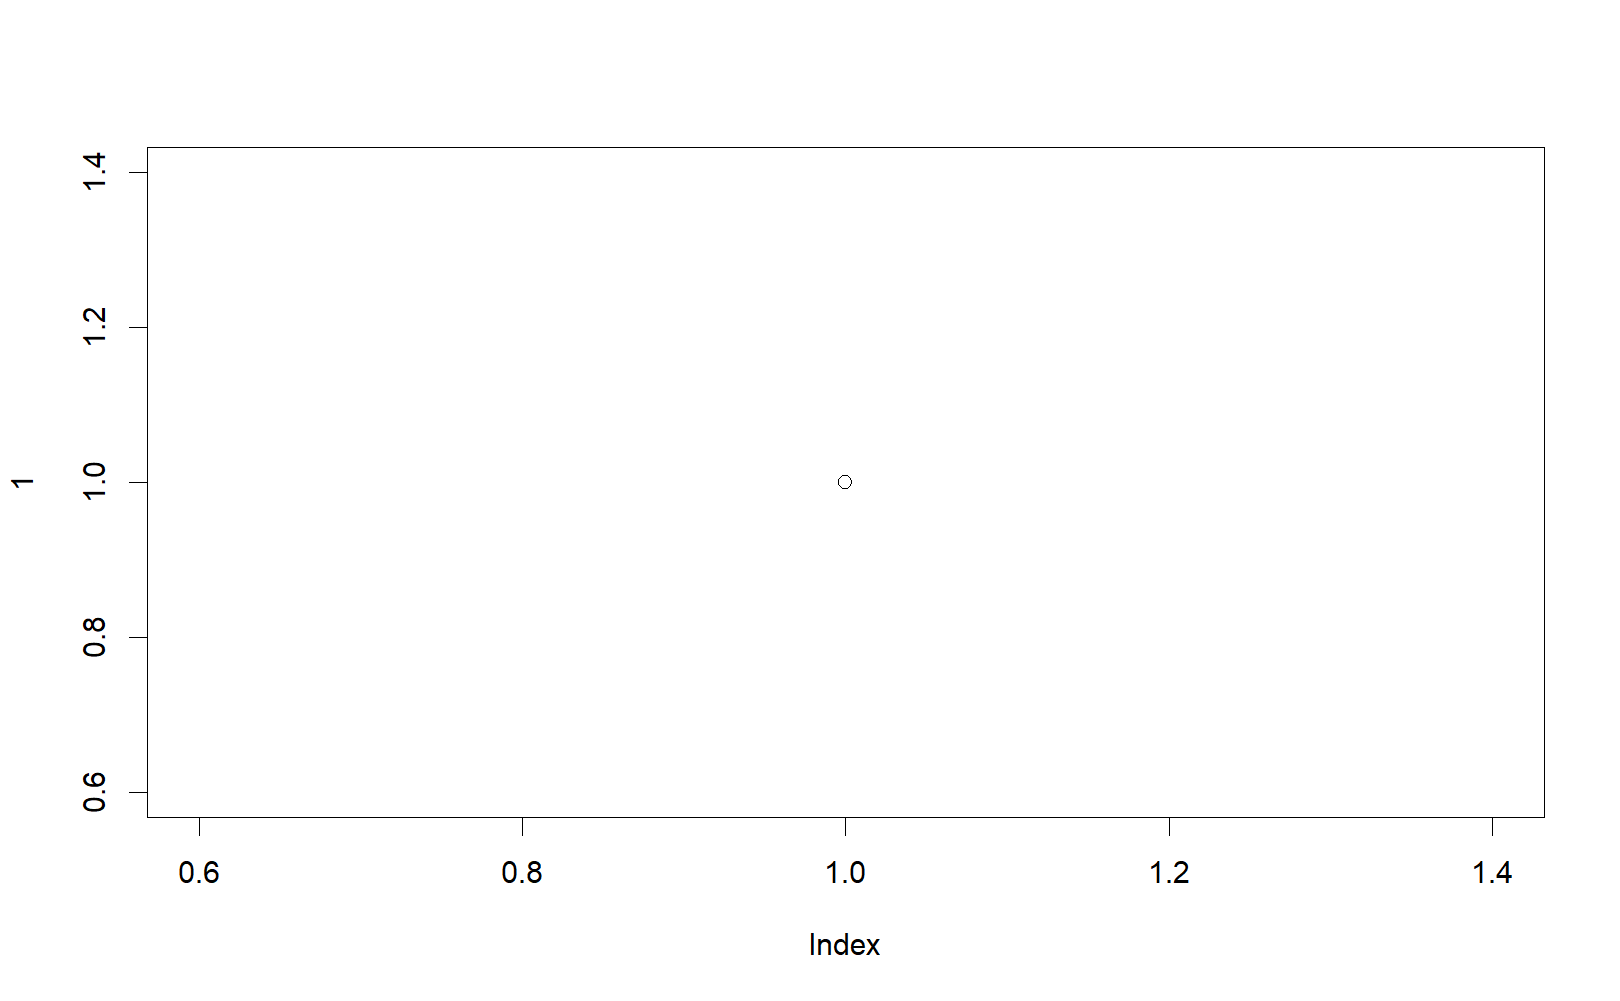
\includegraphics[width=6in]{knitr-figs-pdf/test1-1}}{Figure \ref{fig:test1}} 

}

\caption{Test}\label{fig:test1}
\end{figure}
\begin{longtable}[]{@{}lr@{}}
\caption{\label{tab:test2}Test}\tabularnewline
\toprule
x & y\tabularnewline
\midrule
\endfirsthead
\toprule
x & y\tabularnewline
\midrule
\endhead
a & 1\tabularnewline
a & 2\tabularnewline
b & 3\tabularnewline
\bottomrule
\end{longtable}
\begin{equation}
  1 + 1
  \label{eq:test2}
\end{equation}
See Figure~\ref{fig:test1} for the example appendix figure.

See Table~\ref{tab:test2} for the example appendix table.

\clearpage

\section{THE SECOND APPENDIX, FOR FUN}
\label{app:second-appendix}

More content.

\end{appendices}

\clearpage

\hypertarget{references}{%
\section{References}\label{references}}

\hypertarget{refs}{}
\leavevmode\hypertarget{ref-edwards2013}{}%
Edwards, A.M., Haigh, R., and Starr, P.J. 2014. Pacific Ocean Perch (\emph{Sebastes alutus}) stock assessment for the north and west coasts of Haida Gwaii, British Columbia. DFO Can. Sci. Advis. Sec. Res. Doc. 2013/092: vi + 126 p.
\end{document}
